\documentclass[conference]{IEEEtran}
\IEEEoverridecommandlockouts
% The preceding line is only needed to identify funding in the first footnote. If that is unneeded, please comment it out.
\usepackage{cite}
\usepackage{amsmath,amssymb,amsfonts}
\usepackage{algorithm}
\usepackage{algorithmic}
\usepackage{graphicx}
\usepackage{textcomp}
\usepackage{xcolor}
\usepackage{subfigure}
\usepackage{placeins}
\def\BibTeX{{\rm B\kern-.05em{\sc i\kern-.025em b}\kern-.08em
    T\kern-.1667em\lower.7ex\hbox{E}\kern-.125emX}}
\begin{document}

\title{Niche Radius Adaptation in Bat Algorithm for Locating Multiple Optima in Multimodal Functions\\
% {\footnotesize \textsuperscript{*}Note: Sub-titles are not captured in Xplore and
% should not be used}
% \thanks{Identify applicable funding agency here. If none, delete this.}
}

\author{\IEEEauthorblockN{ Takuya Iwase}
\IEEEauthorblockA{\textit{The Univ. of Electro-Communications} \\
% \textit{name of organization (of Aff.)}\\
Tokyo, Japan \\
tanu\_iwa@cas.lab.uec.ac.jp}
\and
\IEEEauthorblockN{ Ryo Takano}
\IEEEauthorblockA{\textit{The Univ. of Electro-Communications} \\
% \textit{name of organization (of Aff.)}\\
Tokyo, Japan \\
takano@cas.lab.uec.ac.jp}
\and
\IEEEauthorblockN{ Fumito Uwano}
\IEEEauthorblockA{\textit{The Univ. of Electro-Communications} \\
% \textit{name of organization (of Aff.)}\\
Tokyo, Japan \\
uwano@cas.lab.uec.ac.jp}
\and
\IEEEauthorblockN{ Hiroyuki Sato}
\IEEEauthorblockA{\textit{The Univ. of Electro-Communications} \\
% \textit{name of organization (of Aff.)}\\
Tokyo, Japan \\
h.sato@uec.ac.jp}
\and
\IEEEauthorblockN{ Keiki Takadama}
\IEEEauthorblockA{\textit{The Univ. of Electro-Communications} \\
% \textit{name of organization (of Aff.)}\\
Tokyo, Japan \\
keiki@hc.uec.ac.jp}
\and
\IEEEauthorblockN{                      }
% \IEEEauthorblockA{\textit{dept. name of organization (of Aff.)} \\
% \textit{name of organization (of Aff.)}\\
% City, Country \\
% email address}
}

\maketitle

\begin{abstract}
    Evolutionary algorithms (EAs) are often used for multimodal optimization which is modeled as real-world problem. However, most EAs still not enough to find multiple local optima because of the concept of the solution movement between nearest neighbor solutions. This paper proposes the niche radius-based bat algorithm (NRBA), which is designed to find multiple local optima in multimodal optimization.
    We focus on bat algorithm (BA) which deals with the trade-off between exploration and exploitation in the evolutionary process and extend it with niche radius which can control and modify the search space of solutions to avoid overlapping the found optima. In detail, the proposed BA consists of three search phases: (i) the movement from neighbors for avoiding overlapping the same found optima; (ii) the exploitation for searching nearby the best solution of its domain with Niche Radius; (iii) the exploration for searching randomly in all domain of the radius. In order to evaluate the performance of NRBA, this paper employs some test-bed multimodal functions and compare NRBA with BA and NSBA. The experimental results suggest that NRBA is able to provide the better search performance than BA and NSBA to find multiple global optima in most of benchmark functions.
\end{abstract}

\begin{IEEEkeywords}
Bat Algorithm, Multimodal Optimization, Swarm Intelligence
\end{IEEEkeywords}

\section{Introduction}
There are many studies on evolutionary algorithms (EAs) solving the real-world optimization problems which are mostly multimodal and complex optimization problems. These problems has not only single global optimum but also many local optima, hence EAs are required to find the both multiple optima which might be changed their own location as the environment changes. 
% However, most of EAs such as Genetic Algorithm (GA) \cite{GA}, Particle Swarm Optimization (PSO) \cite{PSO01} and Differential Evolution(DE) \cite{DE} designed to converge toward a single global optimum for the static environment, is difficult to find these optima.

To tackle multimodal optimization problems, numerous techniques which are commonly known as \textit{niching methods} have proposed in \cite{Niching}-\cite{EAs02}, \cite{CDE} \cite{SDE}. Thomsen proposed the DE \cite{DE} extends with a crowding scheme (CDE) \cite{CDE} to replace the high-quality solution by the most similar candidate solutions. Li proposed the DE with Speciation (SDE) \cite{SDE} to keep a solution away from the nearest neighbor solution when the distance of both these solutions is less than the threshold. However, these niching methods are still not enough to find multiple local optima because both of them do not consider searching globally though they consider the solution movement according to the euclidean distance between the nearest neighbor solutions. For solving this problem, this paper focuses on Bat Algorithm (BA) that has the characteristic of echolocation which can predict the distance between bats and the target (\textit{i.e., object/food source}). This algorithm enables bats to estimate the distance between their location and the target even in the situations such as the target surrounded by obstacles and the absence of light. Bats can adjust their velocity which is controlled by their loudness, pulse emission rate and frequency, toward the target. While the iteration search step continues until bats reaches the target in the evolutionary process, bats will stop searching the target within its perceptible distance. This research employs BA which copes with exploitation and exploration search, extending with Niche Radius for multimodal optimization. Niche Radius is the threshold distance calculated by the fitness landscape and the number of its peaks.
% In this research, BA is employed because of the following reasons: (1) BA based on the three search phases from (i) to (iii) as described above, while EAs are mainly based on one search phase; and (2) this difference suggests that one of search phases in BA can be modified for finding multiple local optima with keeping the two search phases as original, while the search phase in EAs are hard to be modified for such a purpose due to a lack of the original search phase. What should be noted here is that BA still has the functions of exploitation and exploration in the solution search process as a local search by the phase (ii) and a global search by the phase (iii). Additionally, we extend BA with Niche Radius, which can control and separate the search space of solutions to avoid overlapping the found optima. Niche Radius ***.

This paper is organized as follows. After this section, the mechanism of BA and the proposed algorithm NRBA are explained in Sections 2 and 3. Section 4 describes the multimodal functions as the test-bed problem in the experiment. Section 5 shows the results while Section 6 discusses them. Finally, this paper concludes in Section 7.

\section{Bat Algorithm}
As mentioned in Section 1, BA is a metaheuristic algorithm based on the bat behavior according to its loudness and pulse emission rate of the reflect wave, which control the balance between a local and global search. When a bat finds the better solution than the current one, the loudness $A_i$ and the pulse rate $r_i$ gradually decreases and increases, respectively. To find better solution, the bat has the following three solution search phases: (i) the bat $i$ flies to the target (\textit{i.e.}, the bat which finds the best solution) with the velocity controlled by frequency $f_i$; (ii) the bat $i$ flies around the target as a local search; and (iii) the bat $i$ flies randomly in search space as a global search.
Let us explain these search phases.
First, in the search phase (i), all bats change their locations $x_i$ with their velocities $v_i$ toward the global best solution. For this calculation, the frequency $f_i$, velocity $v_i$, and location $x_i$, of the bat $i$ are calculated as follows:
\begin{equation}
f_{i} =f_{min}+(f_{max}-f_{min}) \beta
\label{eq:freq} 
\end{equation}

\begin{equation}
v_i^{t+1}=v_i^t+(x_*-x_i^t)* f_i
\label{eq:vi}
\end{equation}
\begin{equation}
x_i^{t+1}=x_i^t+v_i^{t+1}
\label{eq:xi}
\end{equation}
In detail, the new solution candidate $x_i$ is updated by adding the new the velocity ${v_i}$ which is derived from the previous velocity $v_i^t$, the distance between the global best location and the previous location $(x_*-x_i^t)$, and frequency $f_i$ which range is [${f_{min}}$, ${f_{max}}$] where ${f_{min}}=0$ and ${f_{max}}=1$. $\beta $ is uniform random value from 0 to 1. Next, in the solution search phase (ii), the new solution candidate $x_{loc}$ is generated around the global best solution as follows:
\begin{equation}
x_{loc}=x_{*}+ \epsilon A^t \ ,
\label{eq:loc}
\end{equation}
where ${\epsilon}$ is uniform random value between ${[0,  \ 1]}$. In Eq.(\ref{eq:A}), ${A^t}$ is the averaged loudness of all bats. Finally, in the search phase (iii), $x_{rnd}$ is generated randomly in search space as follows:
\begin{equation}
\label{eq:xrnd}
x_{rnd}=x_{lb}+(x_{ub}-x_{lb})*rand(1,D)
\end{equation}
where $x_{ub}$ and $x_{lb}$ describe the upper and the lower bounds of the search space, and $rand(1,D)$ is the $D$ dimensional uniform random value between $[0, \ 1]$. 

When a bat finds the better solution than the current one, the loudness $A_i$ and pulse emission rate $r_i$ are updated as follows:
\begin{equation}
A_i^{t+1}=\alpha A_i^t
\label{eq:A}
\end{equation}
\begin{equation}
r_i^{t+1}=r_i^0[1-exp(-\gamma t)]
\label{eq:r}
\end{equation}
Note that the loudness $A_i^0$ is initialized as $A_i^0=1$ and the pulse rate is initialized as a uniform random value $r^0$ between $[0, \ 1]$ or a number closed around zero. The parameters $\alpha$ and $\gamma$ are the symbolized damping coefficient. The pseudo code of BA is given in the Algorithm 1 and its brief summary is described below.

\begin{itemize}
\item STEP1: Population initialization of bats (line 1 to 3)\\
The population of bats ${x_i}(i=1, 2, ..., N)$, the loudness ${A_i^0}$, the pulse rate ${r_i^0}$ are initialized as the initial values. The frequency ${f_i}$ is initialized by Eq.(\ref{eq:freq}).
\item STEP2: New solution updates (line 6)\\
The new solution candidates ${x_i}$ is calculated by Eqs. (\ref{eq:vi}), (\ref{eq:xi}).
\item STEP3: New solution generation around global best solution ${x_*}$ (line 7 to 9)\\
A new solution candidate $x_{loc}$ is generated around $x_*$ by Eq. (\ref{eq:loc}) when the pulse emission rate $r_i$ is lower than a random value.
\item STEP4: Random new solution generation (line 10)\\
A new solution candidate ${x_{rnd}}$ is generated randomly by Eq. (\ref{eq:xrnd}).  
\item STEP5: Solutions update(line 11 to 14)\\
When ${rand < A_i}$, the personal best solution is selected from $x_i$, ${x_{loc}}$, and ${x_{rnd}}$ by Eqs.(\ref{eq:A}),(\ref{eq:r})
\item STEP6: Return to STEP2 
\end{itemize}

\begin{algorithm}[H]
\caption{Bat Algorithm}
\label{code:ba}
\begin{algorithmic}[1]
\REQUIRE Objective\ Function\ $F(x)$
\STATE Initialize Population $x_i(i=1,2,..., N)$ and $v_i$\\
\STATE Define frequency $f_i$ at location $x_i$ [Eq.(\ref{eq:freq})]
\STATE Initialize pulse rates $r_i$, and loudness $A_i$
\WHILE{($t <$ Max number of iterations)}
\FOR{i=1 to N}
\STATE Generate a new solution candidate $x_i$ and velocity $v_i$ [Eqs.(\ref{eq:vi}), (\ref{eq:xi})]
\IF{($rand>r_i$)}
\STATE Generate a new solution candidate $x_{loc}$ around a global best solution $x_i$ [Eq.(\ref{eq:loc})] 
% \ELSE
% \STATE Continue
\ENDIF
\STATE Generate a new solution candidate $x_{rnd}$ randomly
\IF{($rand<A_i \& \min (F(x_i), F(x_{loc}), F(x_{rnd})<F(x_{i*})$)}
\STATE Accept the new solution, and update pulse rate $r_i$ \\ \& loudness $A_i$ [Eqs. (\ref{eq:A}), (\ref{eq:r})]  
\ENDIF
\STATE Evaluate all bats and select a personal best solution $x_{i*}$ in the current solutions
\ENDFOR
\STATE t=t+1
\ENDWHILE
\end{algorithmic}
\end{algorithm}

\section{Proposed Algorithm}
\subsection{Niche Radius}
Niche Radius (NR) \cite{Niche}\cite{DNCMA} is one of niching techniques to determine the radius which is calculated by the number of local optima and the scale of the fitness landscape as follows:
\begin{equation}
\label{eq:lambda}
\lambda =\frac{1}{2} \sqrt{(x_{ub}-x_{lb})^2}
\end{equation}
\begin{equation}
\label{eq:NR}
NR=\frac{\lambda}{\sqrt[D]{q}},
\end{equation}
where the lower and the upper bound values are $x_{ub}$ and $x_{lb}$ of the $D$-th dimensional search space,   and the number of local optima is $q$. Each domain of the radius as $NR$ is wrapping the local optimum to avoid converging same optima.

\subsection{Niche Radius-based Bat Algorithm}
As stated earlier, proposed algorithm is extended BA with the concept of Niche Radius which is able to locate many solutions without converging the found global best solutions within the domain of niche radius. This process is given by
\begin{equation}
\label{eq:nrvi}
v_i^{t+1}=v_i^t+(x_i^t-x_{NR*})*f_i
\end{equation}
\begin{equation}
\label{eq:nrxi}
x_i^{t+1}= \begin{cases}
x_i^t+v_i^{t+1} & (if \ d_i^t < NR) \\
x_i^t & (otherwise)
\end{cases}
\end{equation}
where $x_{NR*}$ is the personal best solution in the domain of niche radius and $d_i^t$ indicates the Euclidean distance between the nearest neighbor solutions. Fig. \ref{fig:niche} provides an example to illustrate the solution movement to keep the solution $x_i$ from the personal best solution $x_{NR*}$ in the domain of the radius, where the red circle and the yellow star indicates solution $x_i$ and the personal best solution $x_{NR*}$. This figure shows the situation that the solutions $x_1, x_2 $ and $ x_3$ are located in the area of $x_{NR*}$ with the radius. In this case, these solutions which are $x_1, x_2$and $x_3$ are moved out from the area of the personal best solution $x_{NR*}$.

\begin{figure}[h]
\begin{center}
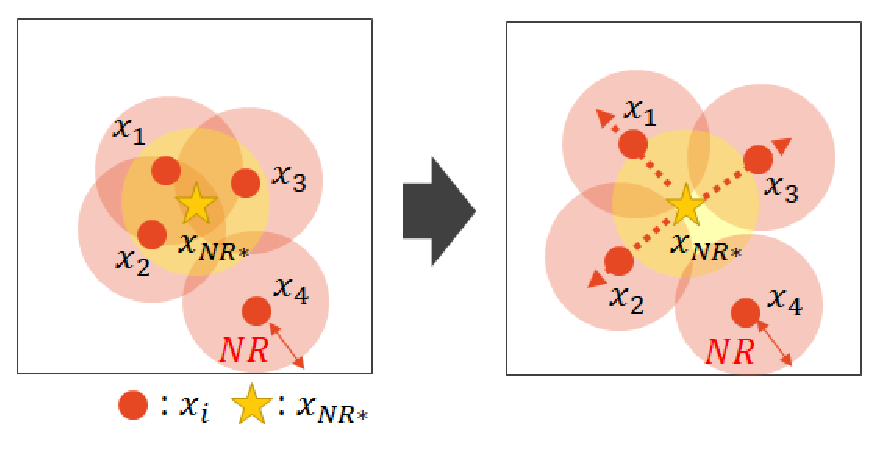
\includegraphics[width=0.8\linewidth]{eps/niche.eps}
\end{center}
\caption{Example of Solution Movement based on Niche Radius}
\label{fig:niche}
\end{figure}

In the local search phase, the new solution candidate $x_{loc}$ is generated around the personal best solution $x_{NR*}$ in the domain of the radius as follows:
\begin{equation}
\label{eq:nrloc}
x_{loc}=x_{NR*} + \epsilon A_i^t
\end{equation}
where $A_i$ and $\epsilon$ is the same values as BA.
In the global search phase, the new solution candidate $x_{rnd}$ is generated randomly in all domains of the range between $[-NR, NR]$ as follows: 
\begin{equation}
\label{eq:nrrnd}
x_{rnd}=x_i^t + rand(1,D,[-NR, NR])
\end{equation}

\subsection{Algorithm Description}
The pseudo code of NRBA is given in Algorithm 2 and its brief summary is described below.
\begin{algorithm}[H]
\caption{Niche Radius-based Bat Algorithm}
\label{code:ba}
\begin{algorithmic}[2]
\REQUIRE Objective\ Function\ $F(x)$
\STATE Initialize Population $x_i(i=1,2,..., N)$ and $v_i$\\
\STATE Define frequency $f_i$ at location $x_i$ [Eq.(\ref{eq:freq})]
\STATE Initialize pulse rates $r_i$, and loudness $A_i$
\WHILE{($t <$ Max number of iterations)}
\FOR{i=1 to N}
\IF{$d_i < NR$ \& $x_i \neq x_{NR*}$}
\STATE Generate a new solution candidate $x_i$ and velocity $v_i$ [Eqs.(\ref{eq:nrvi}), (\ref{eq:nrxi})]
\ENDIF
\IF{($rand>r_i$)}
\STATE Generate a new solution candidate $x_{loc}$ around a global best solution $x_i$ [Eq.(\ref{eq:nrloc})] 
% \ELSE
% \STATE Continue
\ENDIF
\STATE Generate a new solution candidate $x_{rnd}$ randomly [Eq.(\ref{eq:nrrnd})]
\IF{($rand<A_i \& \min (F(x_i), F(x_{loc}), F(x_{rnd})<F(x_{i*})$)}
\STATE Accept the new solution candidate, and update pulse rate $r_i$ \\ \& loudness $A_i$ [Eqs. (\ref{eq:A}), (\ref{eq:r})]  
\ENDIF
\STATE Evaluate all bats and select a personal best solution $x_{i*}$ in the current solutions
\ENDFOR
\STATE t=t+1
\ENDWHILE
\end{algorithmic}
\end{algorithm}

\begin{itemize}
\item STEP1: Population initialization of bats (line 1 to 3)\\
The population of bats ${x_i}(i=1, 2, ..., N)$, the loudness ${A_i^0}$, the pulse rate ${r_i^0}$ are initialized as the initial values. The frequency ${f_i}$ is initialized by Eq.(\ref{eq:freq}).
\item STEP2: New solution updates (line 6 to 8)\\
The new solution candidates ${x_i}$ is calculated by Eqs. (\ref{eq:vi})(\ref{eq:xi}).
\item STEP3: New solution generation around global best solution ${x_*}$ (line 9 to 11)\\
A new solution candidate $x_{loc}$ is generated around $x_*$ by Eq. (\ref{eq:loc}) when the pulse emission rate $r_i$ is lower than a random value.
\item STEP4: Random new solution generation (line 12)\\
A new solution candidate ${x_{rnd}}$ is generated randomly by Eq. (\ref{eq:xrnd}).  
\item STEP5: Solutions update(line 13 to 15)\\
When ${rand < A_i}$, the best solution is selected from $x_i$, ${x_{loc}}$, and ${x_{rnd}}$ by Eqs.(\ref{eq:A}),(\ref{eq:r})
\item STEP6: Return to STEP2 
\end{itemize}

\section{Experiment}
To measure the number of local optima and the convergence speed, we compare with the performance of all algorithms. In this section, four multimodal functions which are considered for maximization, are employed in \textit{Congress on Evolutionary Computation (CEC) 2013} competition on {\it Niching Methods} for
Multimodal Function Optimization \cite{cec2013}. 

\subsection{Experimental setup}
\subsubsection{Benchmark Test Functions}
In order to verify the effectiveness of our proposed algorithm compared with conventional BA and another {\it Niching method} which is Novelty Search-based BA (NSBA) \cite{NSBA}, four benchmark functions that are popular in multimodal optimization are employed in this experiments. The detail of these functions which are the search space, the fitness value of known global optima and the number of known global and local optima, are summarized in Table \ref{tab1}.


\begin{table*}[h]
\caption{Measurement of Benchmark Test Functions}
\begin{center}
\begin{tabular}{c|c|c|c|c}
\hline
Function & ${F_1}$ & ${F_2}$ & ${F_3}$ & ${F_4}$ \\
\hline
Search Space & $x_1, x_2 \in [-6, \ 6]$ & $x_i \in [-10, \ 10]$ & $x_i \in [0.25, \ 10]$ & $x_i \in [0, \ 1]$\\
% & &  & & \\
\hline
Fitness Value & 200.0 & 186.731 & 1.0 & -2.0   \\
\hline
Number of global optima & 4 & 18 & 36 & 12 \\
\hline
Number of local optima &  0 & many & 0 & 0  \\
\hline
accuracy distance $\rho$ & 0.01 & 0.5 & 0.5 & 0.01 \\
\hline
% \multicolumn{4}{l}{$^{\mathrm{a}}$Sample of a Table footnote.}
\end{tabular}
\label{tab1}
\end{center}
\end{table*}

\begin{description}
\item[$F_1$: Himmelblau Function]\mbox{}\\
% This function is described as follows as shown in Fig. \ref{fig:3dgf}.
\begin{equation}
\label{eq:himmelblau}
F_1(x_1,x_2)=200-(x_1^2+x_2-11)^2+(x_1+x_2^2-7)^2
\end{equation}
The fitness value of the global optima is ${F(x_*)}=200$. This function has 4 global optima in the range between $x_1, x_2 \in [-6, \ 6]$.

\begin{figure}[h]
\begin{center}
% \subfigure[Fitness Landscape]{
	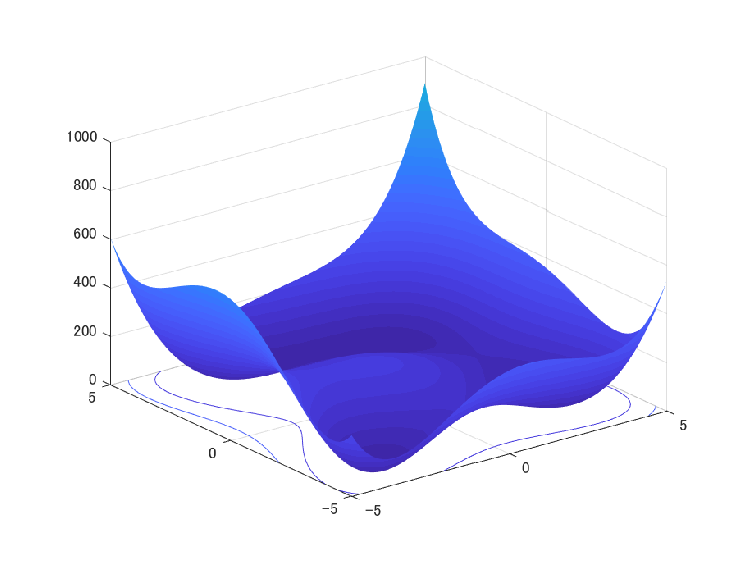
\includegraphics[width=0.8\linewidth]{eps/3d_himmelblau.eps}
% 	\label{fig:3d_himmelblau}
% }
% \subfigure[Contour Plot]{
% 	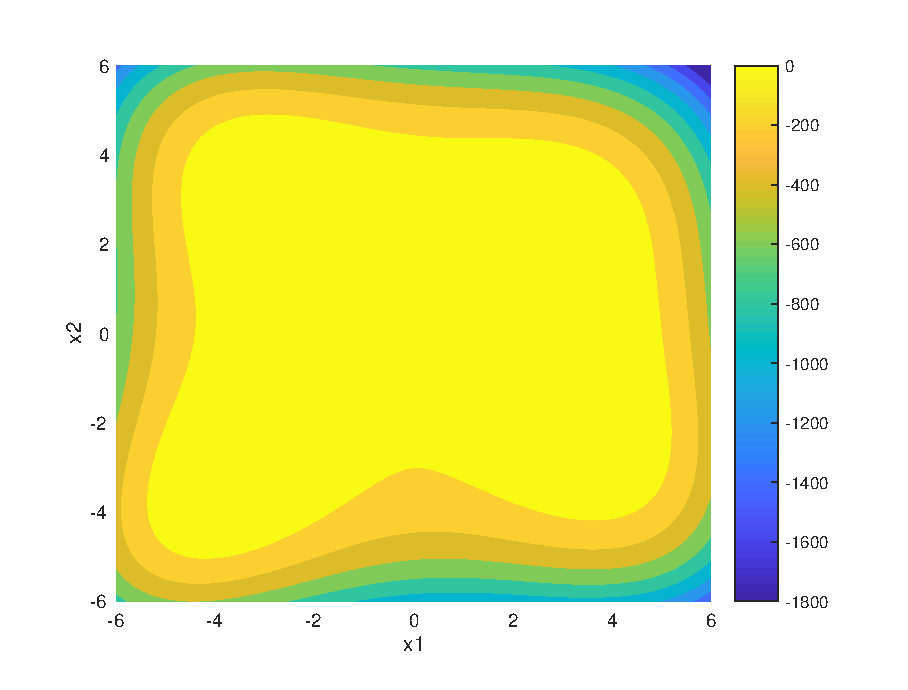
\includegraphics[width=0.8\linewidth]{eps/cont_himmelblau.eps}
% 	\label{fig:cont_himmelblau}
% }
\caption{Himmelblau}
\label{fig:f1}
\end{center}
\end{figure}

\item[$F_2$: Shubert Function]\mbox{}\\
 This function is described as follows as shown in Fig. \ref{fig:f2}.
 \begin{equation}
F_2(x) = -\prod_{i=1}^D \sum_{j=1}^5 j \cos[(j+1)x_i+j], 
\end{equation}
where $D$ is the number of dimension and the fitness value of the global optima is ${F(x_*)=187.731}$. This function has  $D \cdot 3^D $ global optima and numerous local optima in the range of search space between $x_i \in [-10, 10]^D$ with $i=1,2,...,D$. Fig. \ref{fig:f2} shows an example of the Shubert 2D function which has 18 global optima. 

\begin{figure}[h]
\begin{center}
% \subfigure[Fitness Landscape]{
	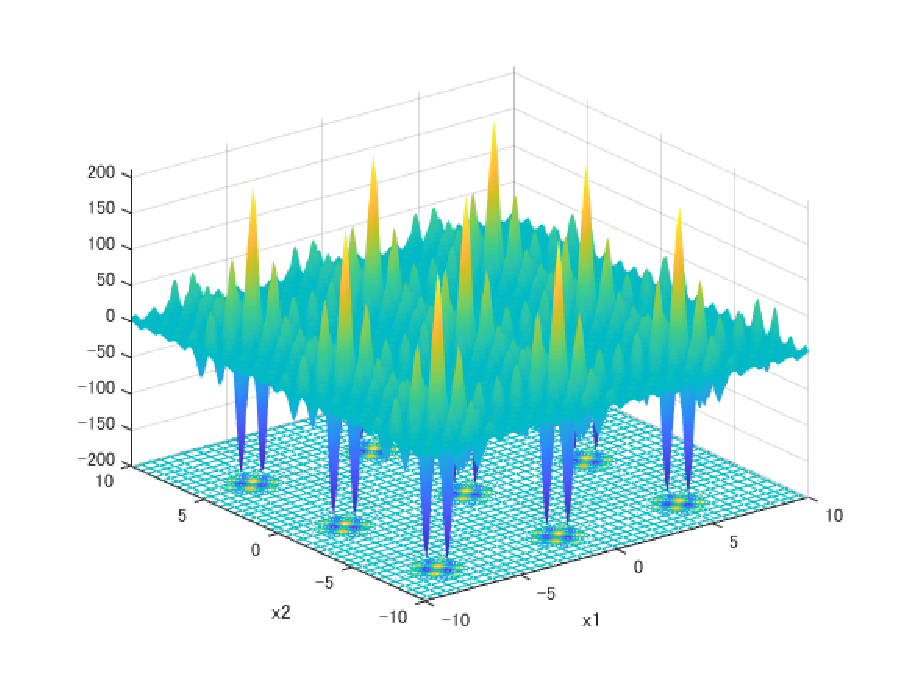
\includegraphics[width=0.8\linewidth]{eps/3d_shubert.eps}
	% \label{fig:3d_shubert}
% }
% \subfigure[Contour Plot]{
% 	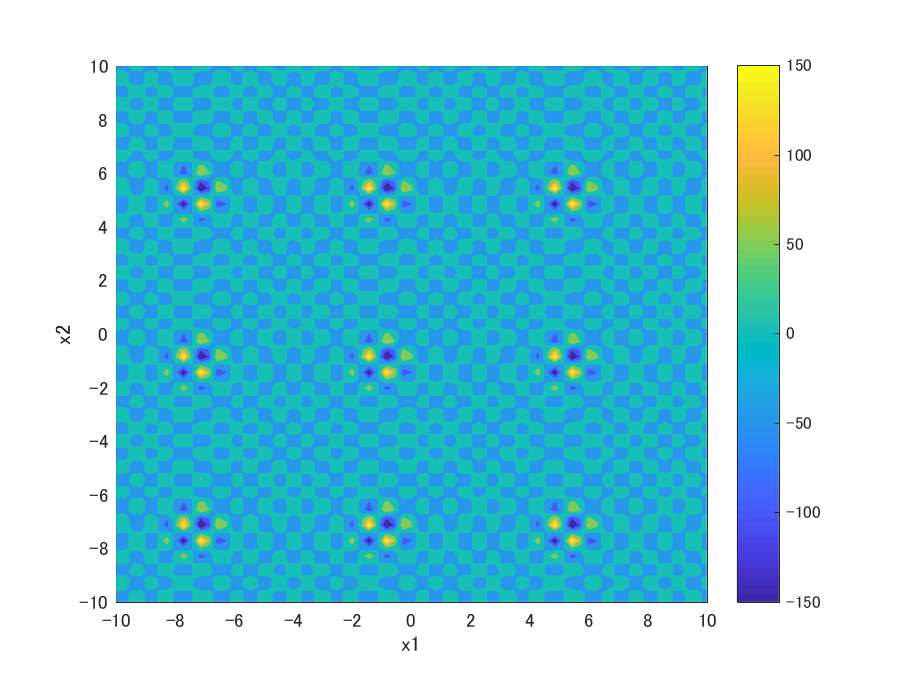
\includegraphics[width=0.8\linewidth]{eps/cont_shubert.eps}
% 	\label{fig:cont_shubert}
% }
\caption{Shubert}
\label{fig:f2}
\end{center}
\end{figure}

\item[$F_3$: Vincent Function]\mbox{}\\
 This function is described as follows as shown in Fig. \ref{fig:f3}.
 \begin{equation}
F_3(x) = \frac{1}{D} \sum_{i=1}^D \sin(10log(x_i)) 
\end{equation}
where $D$ is the number of the dimension and the fitness value of the global optima is ${F(x_*)=1.0}$. This function has $6^D $ global optima in the range of search space between $x_i \in [0.25, 10]^D$ with $i=1,2,...,D$. This figure provides the 2D function in case of 36 global optima with $D=2$. 

\begin{figure}[h]
\begin{center}
% \subfigure[Fitness Landscape]{
	\includegraphics[width=0.8\linewidth]{eps/3d_vincent.eps}
% 	\label{fig:3d_vincent}
% }
% \subfigure[Contour Plot]{
% 	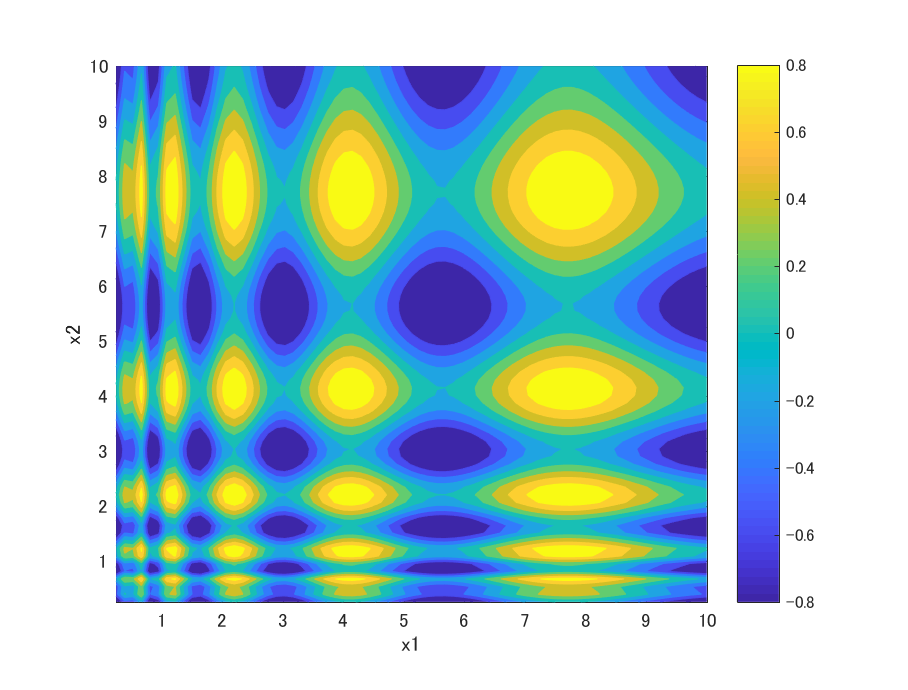
\includegraphics[width=0.8\linewidth]{eps/cont_vincent.eps}
% 	\label{fig:cont_vincent}
% }
\caption{Vincent}
\label{fig:f3}
\end{center}
\end{figure}

\item[$F_4$: Modified Rastrigin Function]\mbox{}\\
 This function is described as follows as shown in Fig. \ref{fig:f4}.
 \begin{equation}
F_4(x) = -\sum_{j=1}^D (10+9 \cos(2 \pi k_i x_i)) 
\end{equation}
where $D$ is the number of dimension and the fitness value of the global optima is ${f(x_*)=-2.0}$. In the case of $D=2$, this function has $\prod_{i=1}^D k_i$ \textit{(12 global optima)} with following setting: $k_1=k_3=1, k_2=4, k_=2$  global optima in the range of search space between $x_i \in [0, 1]^D$ with $i=1,2,...,D$.

\begin{figure}[h]
\begin{center}
% \subfigure[Fitness Landscape]{
	\includegraphics[width=0.8\linewidth]{eps/3d_rastrigin.eps}
% 	\label{fig:3d_rastrigin}
% }
% \subfigure[Contour Plot]{
% 	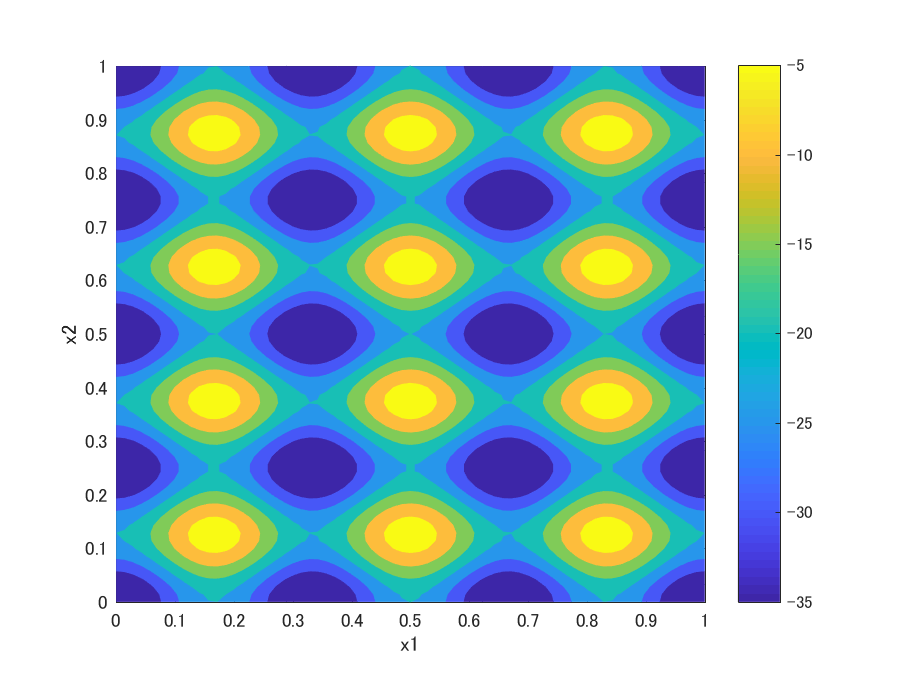
\includegraphics[width=0.8\linewidth]{eps/cont_rastrigin.eps}
% 	\label{fig:cont_rastrigin}
% }
\caption{Modified Rastrigin}
\label{fig:f4}
\end{center}
\end{figure}

\end{description}

\subsubsection{Performance Measurements}
To determine how many global optima the algorithm found, accuracy distance $\rho$ is used to calculate the distance between nearest neighbor individuals as shown in Algorithm \ref{code:foptima}. At the first step, the individuals at the final iteration are sorted by the fitness value in descending order. The next step, if the distance between the fitness of the global optimum $ph$ and the nearest neighbor individual $p$ is less than $\varepsilon$, similar nearest neighbor individuals are compared within accuracy distance $\rho$. The better fitness of individual is added to $S$.

\begin{algorithm}[H]
\caption{Calculate how many global optima the algorithm found}
\label{code:foptima}
\begin{algorithmic}[2]
\REQUIRE $L_{sorted}$ a list of individuals in descending order of the fitness value
\STATE $S = \emptyset$
\WHILE{($not \ reaching \ the \ end \ of \ L_{sorted}$)}
\STATE Get best unprocessed $p \in L_{sorted}$;
\STATE $found \leftarrow$ FALSE;
\IF{$d(ph, fit(p))\leq \varepsilon$}
\FOR{$all \ s \in S$}
\IF{$d(s,p) \leq \rho$}
\STATE $found \leftarrow$ TRUE;
\STATE break;
\ENDIF
\ENDFOR
\IF{not found}
\STATE let $s \leftarrow S \cup \{p\}$
\ENDIF
\ENDIF
\ENDWHILE
\end{algorithmic}
\end{algorithm}

%\begin{description}
%\item Peak Ratio\\
This experiment employs Peak Ratio(PR) \cite{CDE} as the evaluation criterion in the CEC (IEEE Congress on Evolutionary Computation) 2013 competition \cite{cec2013}. The PR value measures the ratio of the found global and local optima in the total number of true peaks and it is calculated as follows: 
\begin{equation}
\label{eq:PR}
PR=\frac{\sum_{run=1}^{MR}FPs}{TP*MR}
\end{equation}
 where ${MR}$ indicates the maximum run, ${FPs}$ indicates indicates the number of peaks found by the optimization algorithm. ${TP}$ indicates the number of all known peaks of the function. We define that the peak is found when the Euclid distance between the all known peaks and the nearest solution calculated by the optimization algorithm is less than the thresholds $\varepsilon = \{1.0, 1.0E-1, 1.0E-2\}$.

%\item Peak Accuracy\\
To measure how far solutions are close to the peaks, we employ Peak Accuracy (PA) \cite{CDE} calculated as follows:
\begin{equation}
PA=\sum_{j=1}^{TP}|F(s_j)-F(x_{NN_j})|,
\end{equation}
where $s_j$ and $x_{NN_j}$ denote the each known peak and the nearest neighbor solution. As the closest distance between both of them is short, the value of PA is close to 0.  
%\end{description}

 \subsubsection{Experimental Parameters}
All experiments employ the parameters as follows: frequency ${f_{max}=1, f_{min}=0}$, loudness ${A^0}=1$, parse rate ${r^0} \in [0, \ 1]$ with ${\alpha =\gamma = 0.9}$. The population size ${N=100}$. This experiments are simulated 30 runs with different random seeds and 10000 evaluations as the termination condition for each run.

% \subsection{Comparison to other Algorithms}

\section{Results and Analysis}
To test the effectiveness of NRBA mechanism, this section investigates the peak ratio (PR) and the peak accuracy (PA) of each benchmark test function. Table \ref{tab2}, \ref{tab3}, and \ref{tab4} show the results that the PR and the PA values of two algorithms based on the settings of averaged over 30 individual runs at the final iteration. Fig. \ref{fig:results_ba} and \ref{fig:results_nrba} show that the solutions relocating and exploiting at the final iteration for all functions.

\begin{figure}[h]
\centering
\subfigure[$F_1$]{
	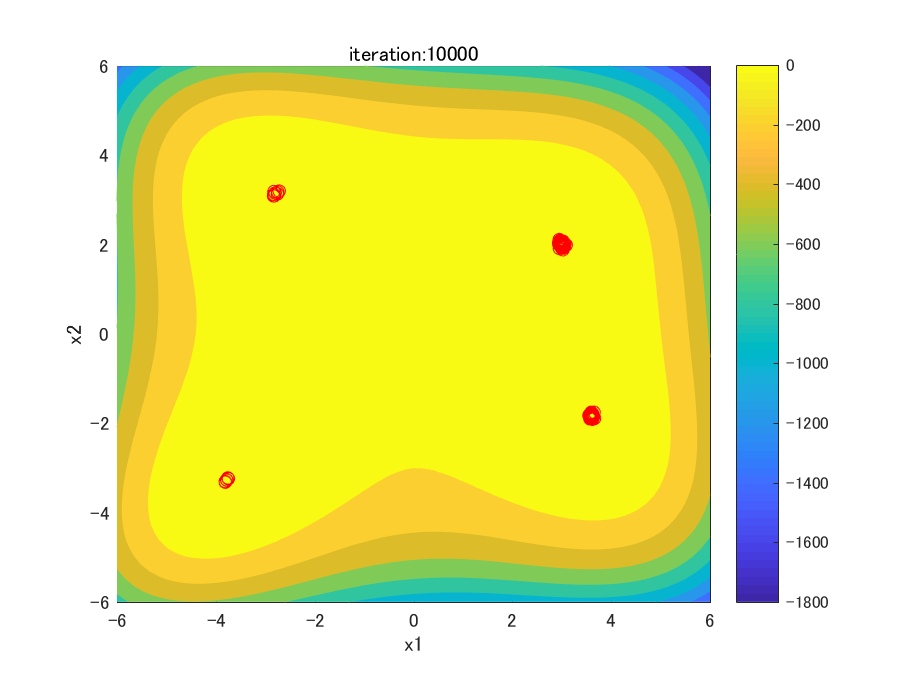
\includegraphics[width=0.8\linewidth]{eps/f1_ba.eps}
	\label{fig:f1_ba}
}
\subfigure[$F_2$]{
	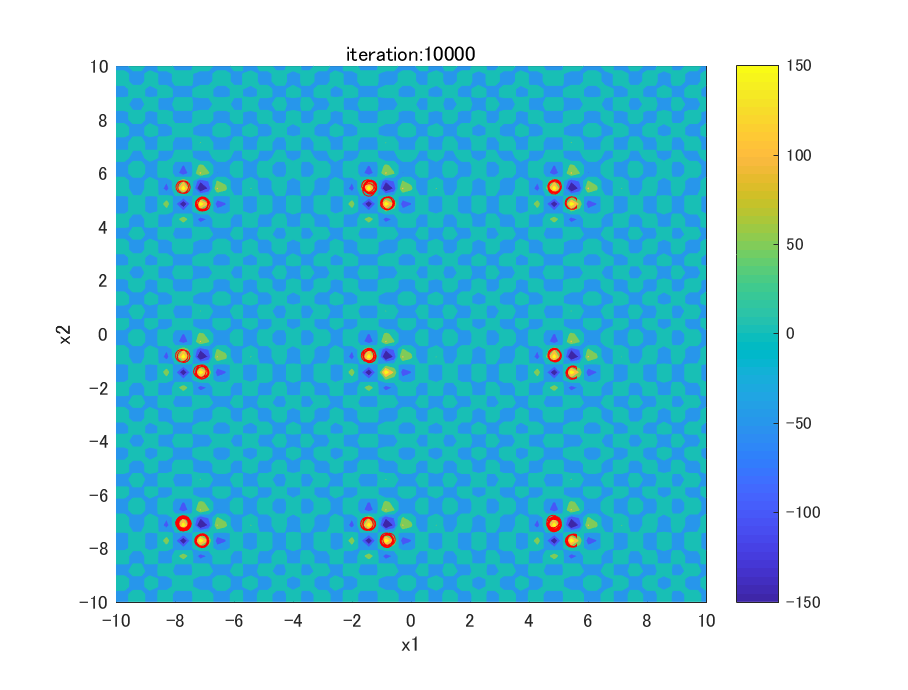
\includegraphics[width=0.8\linewidth]{eps/f2_ba.eps}
	\label{fig:f2_ba}
}
\subfigure[$F_3$]{
	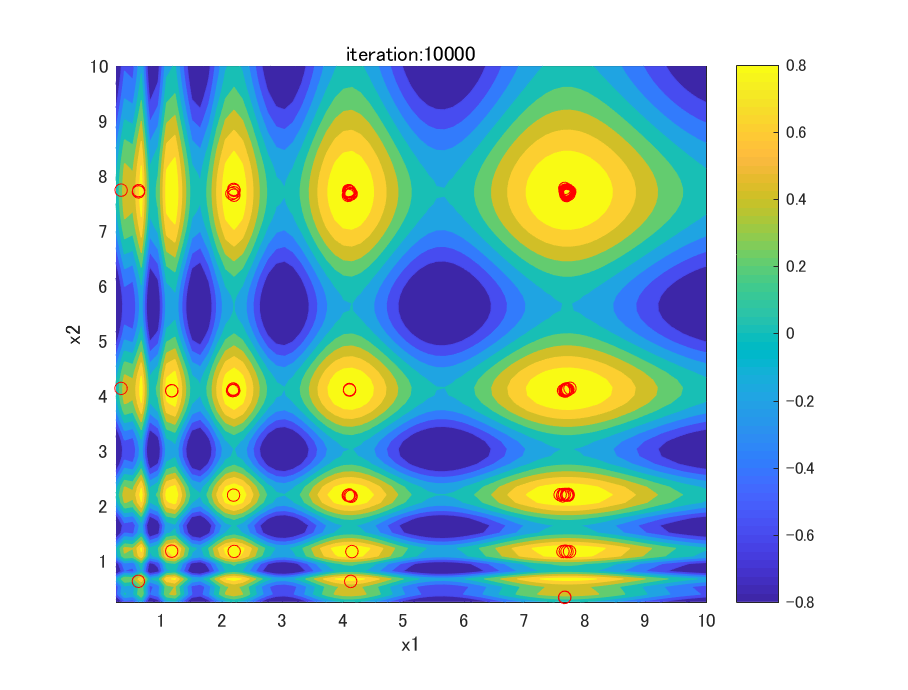
\includegraphics[width=0.8\linewidth]{eps/f3_ba.eps}
	\label{fig:f3_ba}
}
\subfigure[$F_4$]{
	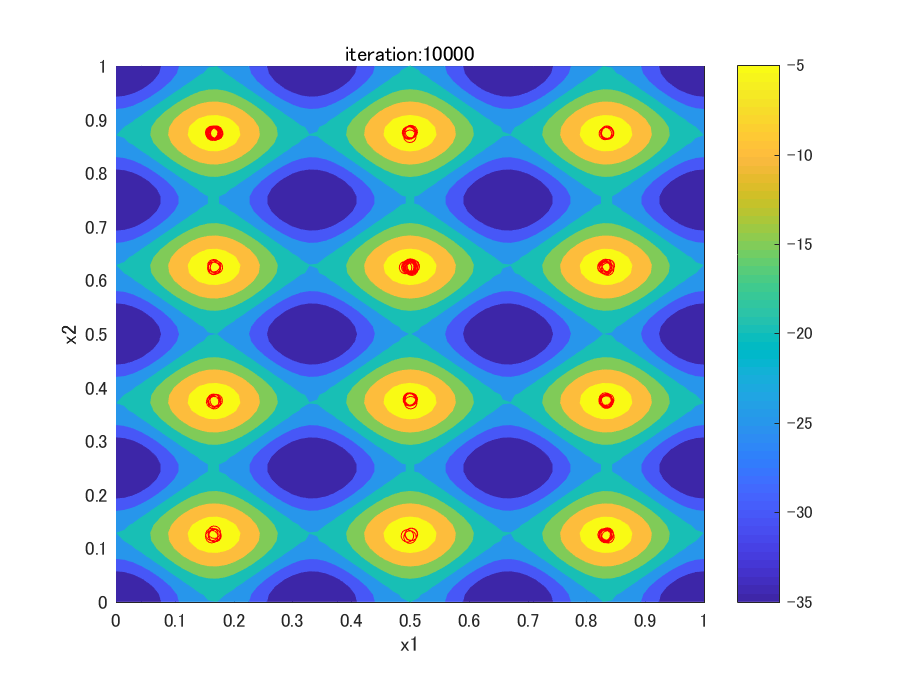
\includegraphics[width=0.8\linewidth]{eps/f4_ba.eps}
	\label{fig:f4_ba}
}
\caption{BA}
\label{fig:results_ba}
\end{figure}
\begin{figure}[h]
\centering
\subfigure[$F_1$]{
	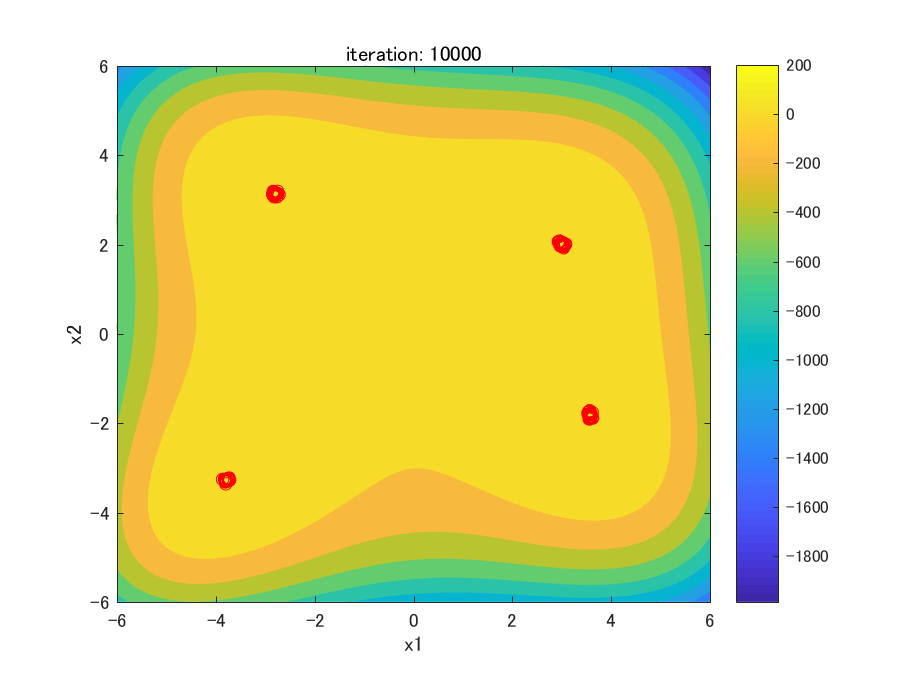
\includegraphics[width=0.8\linewidth]{eps/f1_nsba.eps}
	\label{fig:f1_nsba}
}
\subfigure[$F_2$]{
	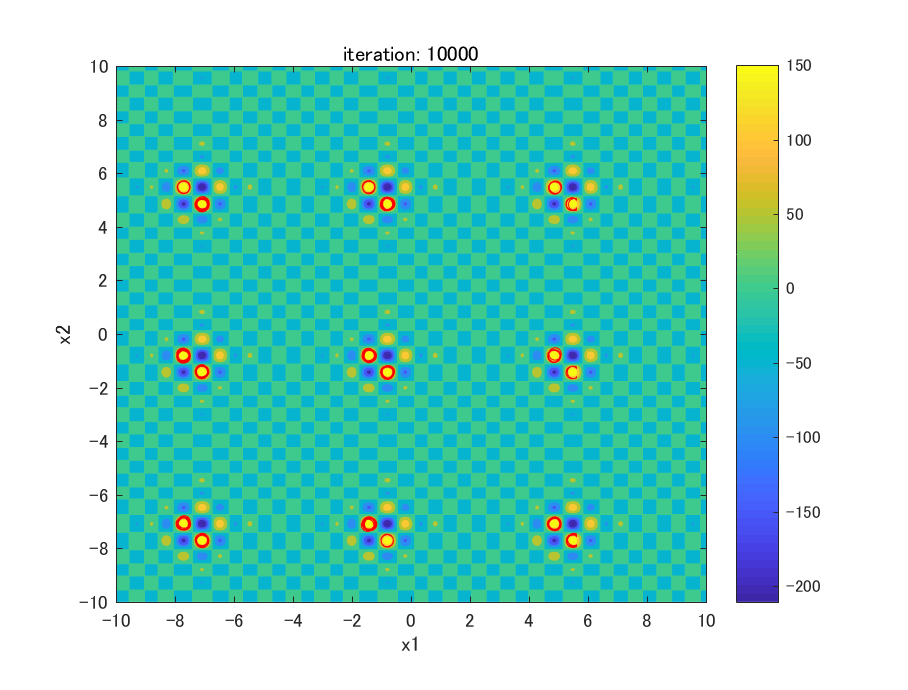
\includegraphics[width=0.8\linewidth]{eps/f2_nsba.eps}
	\label{fig:f2_nsba}
}
\subfigure[$F_3$]{
	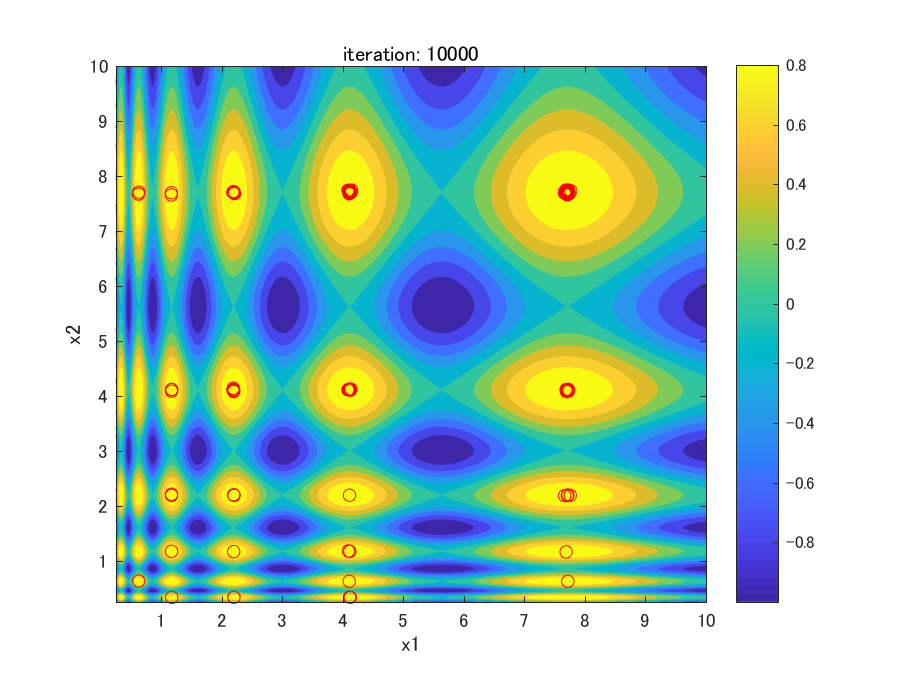
\includegraphics[width=0.8\linewidth]{eps/f3_nsba.eps}
	\label{fig:f3_nsba}
}
\subfigure[$F_4$]{
	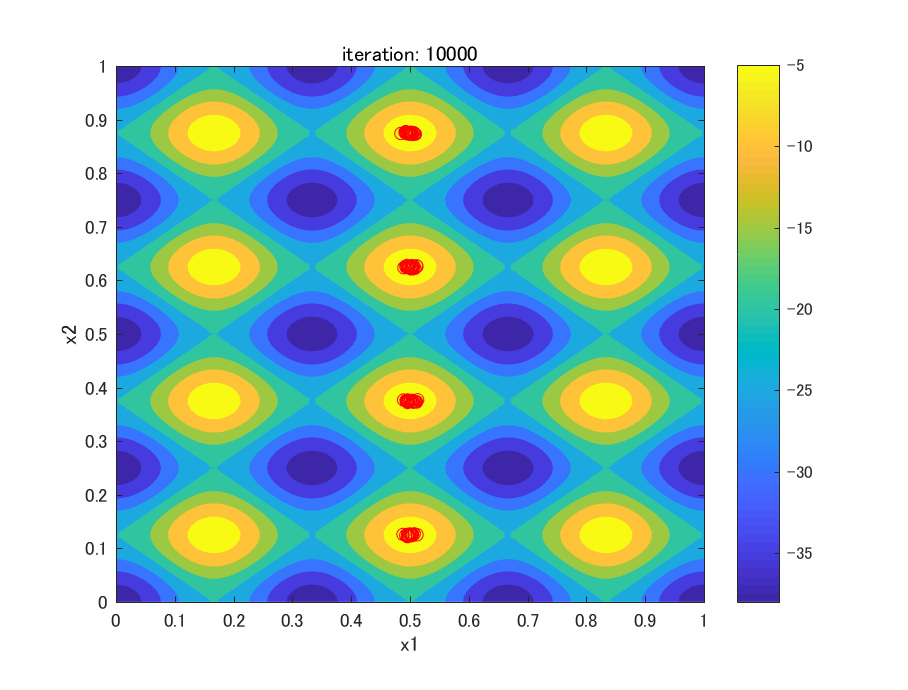
\includegraphics[width=0.8\linewidth]{eps/f4_nsba.eps}
	\label{fig:f4_nsba}
}
\caption{NSBA}
\label{fig:results_nsba}
\end{figure}

\begin{figure}[h]
\centering
\subfigure[$F_1$]{
	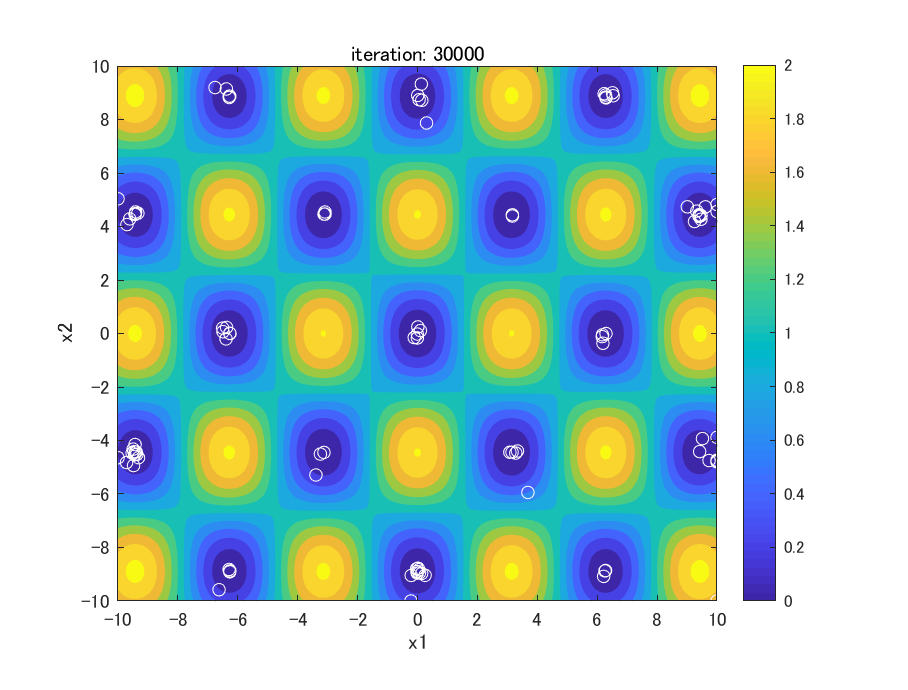
\includegraphics[width=0.8\linewidth]{eps/f1_nrba.eps}
	\label{fig:f1_nrba}
}
\subfigure[$F_2$]{
	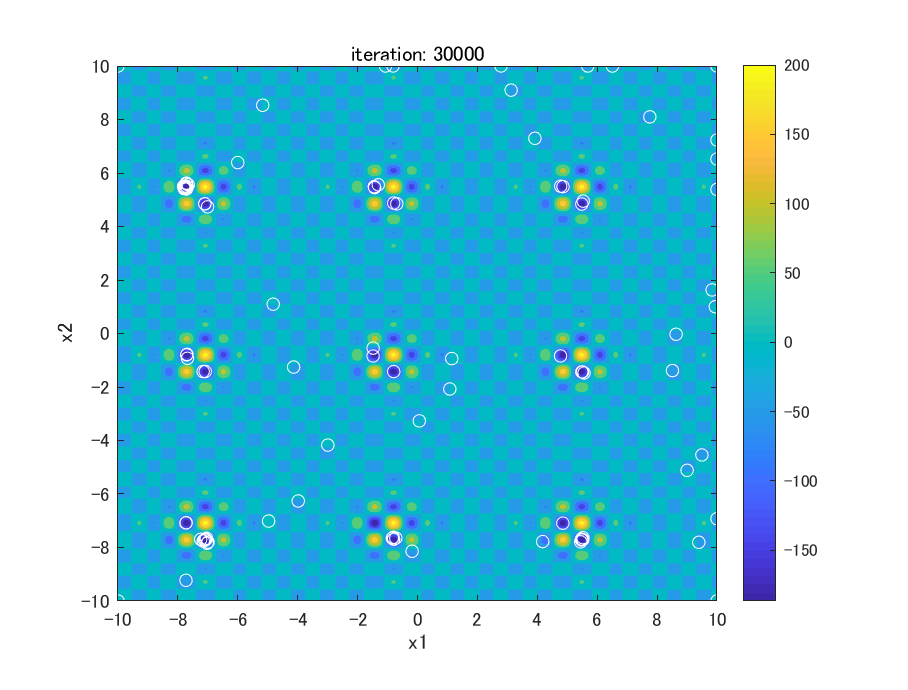
\includegraphics[width=0.8\linewidth]{eps/f2_nrba.eps}
	\label{fig:f2_nrba}
}
\subfigure[$F_3$]{
	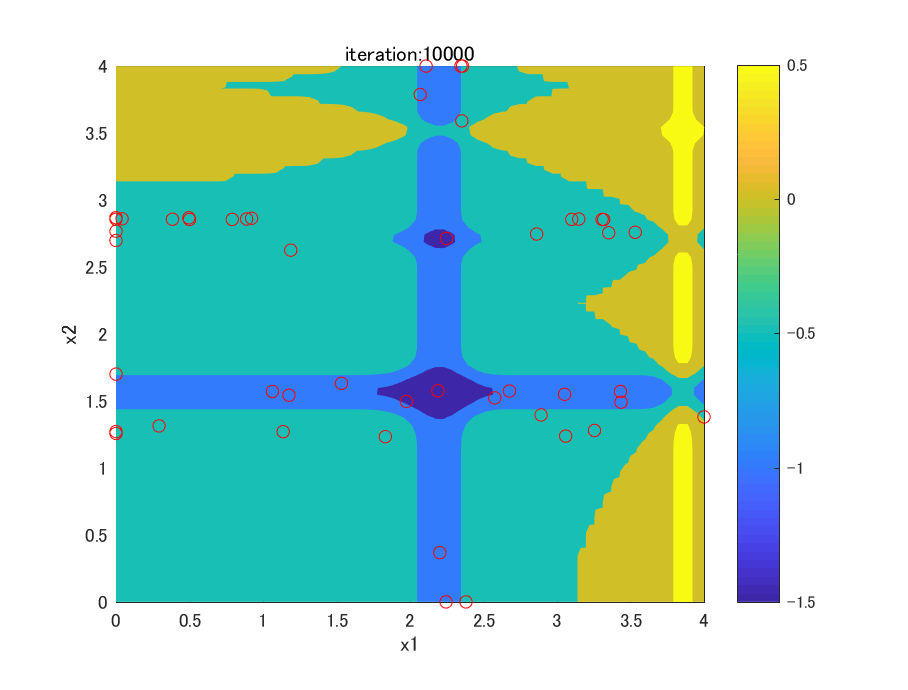
\includegraphics[width=0.8\linewidth]{eps/f3_nrba.eps}
	\label{fig:f3_nrba}
}
\subfigure[$F_4$]{
	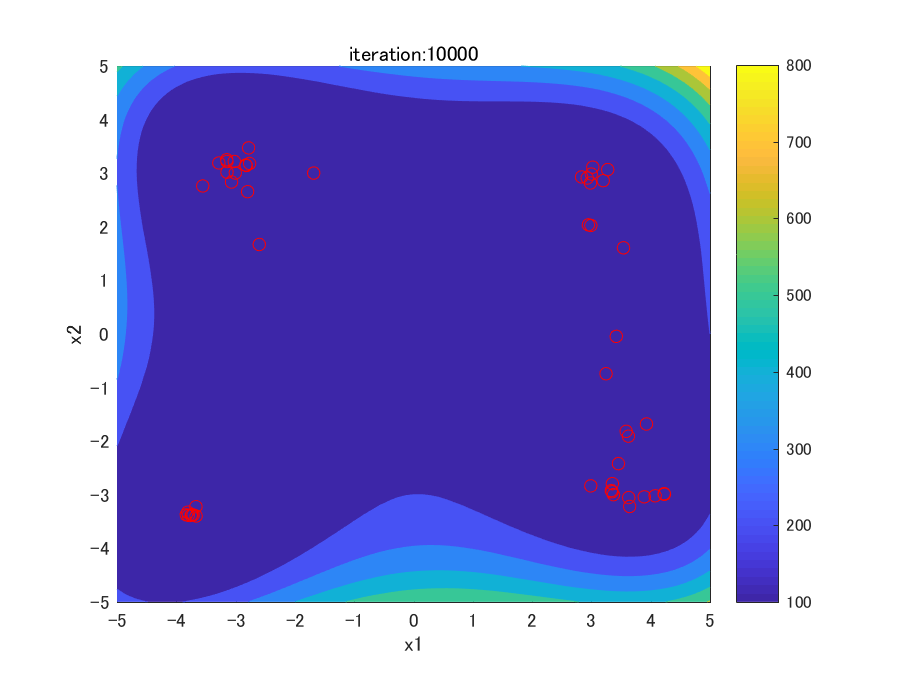
\includegraphics[width=0.8\linewidth]{eps/f4_nrba.eps}
	\label{fig:f4_nrba}
}
\caption{NRBA}
\label{fig:results_nrba}

\end{figure}
% \FloatBarrier

\begin{table*}[h]
\caption{Peak Ratio and Peak Accuracy of BA and NRBA (averaged over 30 runs)}
\begin{center}
\begin{tabular}{c|c|c|c|c|c|c}
\multicolumn{7}{c}{ accuracy level: $\varepsilon = 1.0$} \\
\hline
\multicolumn{1}{c|}{} & \multicolumn{2}{c|}{BA} & \multicolumn{2}{c|}{NSBA} & \multicolumn{2}{c}{NRBA} \\
\hline
 & PR & PA & PR & PA & PR & PA \\

Function & (Mean and SD) & (Mean and SD) & (Mean and SD) & (Mean and SD) & (Mean and SD) & (Mean and SD)  \\
\hline
$F_1 $ & {\bf 1} $\pm$ 0 & {\bf 0.0060} $\pm$ 0.0028 & {\bf 1} $\pm$ 0 & 0.0071 $\pm$ 0.0031 & {\bf 1} $\pm$ 0  & 0.0326 $\pm$ 0.017  \\
\hline
$F_2 $ & 0.5870 $\pm$ 0.0991 & {\bf 3.9272} $\pm$ 1.199 & {\bf 0.8148} $\pm$ 0.0763 & 5.0605 $\pm$ 1.1713 &  0.7111 $\pm$ 0.1077 & 4.765 $\pm$ 1.3987 \\
\hline
$F_3 $ & 0.4407 $\pm$ 0.0839 & {\bf 0.0044} $\pm$ 0.0021 & 0.5963 $\pm$ 0.0530 & 0.0066 $\pm$ 0.0019 & {\bf 0.6685} $\pm$ 0.0699 & 0.0080 $\pm$ 0.0027 \\
\hline
$F_4 $ & 0.9833 $\pm$ 0.0333  & {\bf 0.0287} $\pm$ 0.0102 & 0.0199 $\pm$ 0.0022 & 2.4686 $\pm$ 0.4510 & {\bf 1} $\pm$ 0 & 0.029 $\pm$ 0.0097 \\
\hline
\end{tabular}
\label{tab2}
\end{center}
\end{table*}

\begin{table*}[h]
\caption{Peak Ratio and Peak Accuracy of BA and NRBA (averaged over 30 runs)}
\begin{center}
\begin{tabular}{c|c|c|c|c|c|c}
\multicolumn{7}{c}{accuracy level: $\varepsilon = 1.0E-1$} \\
\hline
\multicolumn{1}{c|}{} & \multicolumn{2}{c|}{BA} & \multicolumn{2}{c|}{NSBA} & \multicolumn{2}{c}{NRBA} \\
\hline
 & PR & PA & PR & PA & PR & PA \\

Function & (Mean and St. D.) & (Mean and St. D.) & (Mean and St. D.) & (Mean and St. D.) & (Mean and St. D.) & (Mean and St. D.) \\
\hline
$F_1 $ & {\bf 1} $\pm$ 0 & {\bf 0.0060} $\pm$ 0.0028 & {\bf 1} $\pm$ 0 & 0.0071 $\pm$ 0.0031 & {\bf 1} $\pm$ 0 & 0.0326 $\pm$ 0.0170  \\
\hline
$F_2 $ & 0.1148 $\pm$ 0.0640 & {\bf 0.0808} $\pm$ 0.0629 & 0.2 $\pm$ 0.0985 & 0.1664 $\pm$ 0.0955 & {\bf 0.1185} $\pm$ 0.0821 & 0.1135 $\pm$ 0.0922 \\
\hline
$F_3 $ &  0.4407 $\pm$ 0.0839 & {\bf 0.0044} $\pm$ 0.0021 & 0.5963 $\pm$ 0.0530 & 0.0066 $\pm$ 0.0016 & {\bf 0.6685} $\pm$ 0.0699 & 0.0081 $\pm$ 0.0027\\
\hline
$F_4 $ & 0.9833 $\pm$ 0.0333 & {\bf 0.0287} $\pm$ 0.0102 & 0.0046 $\pm$ 0 & 0.0555 $\pm$ 0.0140 & {\bf 1} $\pm$ 0 & 0.029 $\pm$ 0.0097 \\
\hline
\end{tabular}
\label{tab3}
\end{center}
\end{table*}

\begin{table*}[h]
\caption{Peak Ratio and Peak Accuracy of BA and NRBA (averaged over 30 runs)}
\begin{center}
\begin{tabular}{c|c|c|c|c|c|c}
\multicolumn{7}{c}{$\varepsilon = 1.0E-2$} \\
\hline
\multicolumn{1}{c|}{} & \multicolumn{2}{c|}{BA} & \multicolumn{2}{c|}{NSBA} & \multicolumn{2}{c}{NRBA} \\
\hline
 & PR & PA & PR & PA & PR & PA \\

Function & (Mean and St. D.) & (Mean and St. D.) & (Mean and St. D.) & (Mean and St. D.) & (Mean and St. D.) & (Mean and St. D.) \\
\hline
$F_1 $ & {\bf 1} $\pm$ 0 & {\bf 0.0060} $\pm$ 0.0028 & {\bf 1} $\pm$ 0 & 0.0071 $\pm$ 0.0031 & 0.6917 $\pm$ 0.3006 & 0.0127 $\pm$ 0.0076  \\
\hline
$F_2 $ & {\bf 0.0315} $\pm$ 0.04223 & 0.0029 $\pm$ 0.0040 & 0.0296 $\pm$ 0.0379 & 0.0026 $\pm$ 0.0044 & 0.0167 $\pm$ 0.0255 & {\bf 0.0020} $\pm$ 0.0034 \\
\hline
$F_3 $ & 0.4407 $\pm$ 0.0839 & {\bf 0.0044} $\pm$ 0.0021 & 0.5963 $\pm$ 0.0530 & 0.0066 $\pm$ 0.0016 & {\bf 0.6685} $\pm$ 0.0699 & 0.0078 $\pm$ 0.0031 \\
\hline
$F_4 $ & 0.9444 $\pm$ 0.0583 & {\bf 0.0215} $\pm$ 0.0069 & NaN & NaN & {\bf 0.9806} $\pm$ 0.0352 & 0.0234 $\pm$ 0.0074 \\
\hline
\end{tabular}
\label{tab4}
\end{center}
\end{table*}



\subsection{Peak Ratio}
From Table \ref{tab2} in the case of $\varepsilon = 1.0$, NRBA has outperformed than the other algorithms for almost all test functions. For $F_1$, the PR value of NRBA was the same as the other algorithms. It can see from this table, all algorithms are able to locate all global optima for all runs (as shown in Fig. \ref{fig:f1_ba} \ref{fig:f1_nsba} and \ref{fig:f1_nrba}. The case of $\varepsilon=1.0E-1$ from Table \ref{tab3}, the PR values of NRBA were also higher than BA and NSBA. However, the values of both algorithms went down greatly from Table \ref{tab2} to \ref{tab3} because $F_2$ is extremely sharp and complex landscape compared with the other functions. Table \ref{tab4} shows that NRBA has outperformed than BA and NSBA in $F_3$ and $F_4$ in the case of $\varepsilon = 1.0E-2$. The performance of NRBA gradually decreased from Table \ref{tab2} to \ref{tab4}. As it can be seen in this table, NRBA was eventually worse than BA and NSBA in $F_1$ and $F_2$. 

\subsection{Peak Accuracy}
NRBA is worse than BA and NSBA for all functions from all Table \ref{tab2}, \ref{tab3} and \ref{tab4} except for $F_2$ in $\varepsilon=1.0E-2$. As it can be seen the results, the exploit phase of BA has worked well more than NRBA regardless of the difference value of threshold $\varepsilon$ from Table \ref{tab2}, \ref{tab3} and \ref{tab4}. Furthermore, the random search phase of BA is assumed to cope with the exploitation and the exploration. However, the density distribution of the solutions is unbalanced (especially in Fig. \ref{fig:f1_ba} and \ref{fig:f3_ba}) due to promoting all solutions to exploit the global best solution. In contrast, NRBA is able to spread the solutions to multiple optima even if some global optima are located the same domain of Niche Radius.

\section{Conclusion}
This paper proposes BA extending with Niche Radius which enables to avoid overlapping the solutions into the same peak and locate multiple global optima in several multimodal functions which are different from landscape and the number of peaks. For solving multimodal optimization, we improved the three search phases of BA: (i) the movement from neighbors for avoiding overlapping the same found optima; (ii) the exploitation for searching nearby the best solution of its domain with Niche Radius; (iii) the exploration for searching randomly in all domain of the radius. To evaluate the performance of NRBA, this algorithm were compared with BA and NSBA. The results show that NRBA performed better than the other algorithms because the spatial distribution mechanism in NRBA copes with locating many multiple global optima. In contrast, BA and NSBA are still better than NRBA regarding the peak accuracy which indicates how far the peaks are close to the solutions, due to the distribution mechanism of NRBA.

In the future, we will improve the algorithm performances: the exploration for searching all global optima completely, and the exploitation for locating global optima rapidly.
% \subsection{Maintaining the Integrity of the Specifications}

% The IEEEtran class file is used to format your paper and style the text. All margins, 
% column widths, line spaces, and text fonts are prescribed; please do not 
% alter them. You may note peculiarities. For example, the head margin
% measures proportionately more than is customary. This measurement 
% and others are deliberate, using specifications that anticipate your paper 
% as one part of the entire proceedings, and not as an independent document. 
% Please do not revise any of the current designations.

% \section{Prepare Your Paper Before Styling}
% Before you begin to format your paper, first write and save the content as a 
% separate text file. Complete all content and organizational editing before 
% formatting. Please note sections \ref{AA}--\ref{SCM} below for more information on 
% proofreading, spelling and grammar.

% Keep your text and graphic files separate until after the text has been 
% formatted and styled. Do not number text heads---{\LaTeX} will do that 
% for you.

% \subsection{Abbreviations and Acronyms}\label{AA}
% Define abbreviations and acronyms the first time they are used in the text, 
% even after they have been defined in the abstract. Abbreviations such as 
% IEEE, SI, MKS, CGS, ac, dc, and rms do not have to be defined. Do not use 
% abbreviations in the title or heads unless they are unavoidable.

% \subsection{Units}
% \begin{itemize}
% \item Use either SI (MKS) or CGS as primary units. (SI units are encouraged.) English units may be used as secondary units (in parentheses). An exception would be the use of English units as identifiers in trade, such as ``3.5-inch disk drive''.
% \item Avoid combining SI and CGS units, such as current in amperes and magnetic field in oersteds. This often leads to confusion because equations do not balance dimensionally. If you must use mixed units, clearly state the units for each quantity that you use in an equation.
% \item Do not mix complete spellings and abbreviations of units: ``Wb/m\textsuperscript{2}'' or ``webers per square meter'', not ``webers/m\textsuperscript{2}''. Spell out units when they appear in text: ``. . . a few henries'', not ``. . . a few H''.
% \item Use a zero before decimal points: ``0.25'', not ``.25''. Use ``cm\textsuperscript{3}'', not ``cc''.)
% \end{itemize}

% \subsection{Equations}
% Number equations consecutively. To make your 
% equations more compact, you may use the solidus (~/~), the exp function, or 
% appropriate exponents. Italicize Roman symbols for quantities and variables, 
% but not Greek symbols. Use a long dash rather than a hyphen for a minus 
% sign. Punctuate equations with commas or periods when they are part of a 
% sentence, as in:
% \begin{equation}
% a+b=\gamma\label{eq}
% \end{equation}

% Be sure that the 
% symbols in your equation have been defined before or immediately following 
% the equation. Use ``\eqref{eq}'', not ``Eq.~\eqref{eq}'' or ``equation \eqref{eq}'', except at 
% the beginning of a sentence: ``Equation \eqref{eq} is . . .''

% \subsection{\LaTeX-Specific Advice}

% Please use ``soft'' (e.g., \verb|\eqref{Eq}|) cross references instead
% of ``hard'' references (e.g., \verb|(1)|). That will make it possible
% to combine sections, add equations, or change the order of figures or
% citations without having to go through the file line by line.

% Please don't use the \verb|{eqnarray}| equation environment. Use
% \verb|{align}| or \verb|{IEEEeqnarray}| instead. The \verb|{eqnarray}|
% environment leaves unsightly spaces around relation symbols.

% Please note that the \verb|{subequations}| environment in {\LaTeX}
% will increment the main equation counter even when there are no
% equation numbers displayed. If you forget that, you might write an
% article in which the equation numbers skip from (17) to (20), causing
% the copy editors to wonder if you've discovered a new method of
% counting.

% {\BibTeX} does not work by magic. It doesn't get the bibliographic
% data from thin air but from .bib files. If you use {\BibTeX} to produce a
% bibliography you must send the .bib files. 

% {\LaTeX} can't read your mind. If you assign the same label to a
% subsubsection and a table, you might find that Table I has been cross
% referenced as Table IV-B3. 

% {\LaTeX} does not have precognitive abilities. If you put a
% \verb|\label| command before the command that updates the counter it's
% supposed to be using, the label will pick up the last counter to be
% cross referenced instead. In particular, a \verb|\label| command
% should not go before the caption of a figure or a table.

% Do not use \verb|\nonumber| inside the \verb|{array}| environment. It
% will not stop equation numbers inside \verb|{array}| (there won't be
% any anyway) and it might stop a wanted equation number in the
% surrounding equation.

% \subsection{Some Common Mistakes}\label{SCM}
% \begin{itemize}
% \item The word ``data'' is plural, not singular.
% \item The subscript for the permeability of vacuum $\mu_{0}$, and other common scientific constants, is zero with subscript formatting, not a lowercase letter ``o''.
% \item In American English, commas, semicolons, periods, question and exclamation marks are located within quotation marks only when a complete thought or name is cited, such as a title or full quotation. When quotation marks are used, instead of a bold or italic typeface, to highlight a word or phrase, punctuation should appear outside of the quotation marks. A parenthetical phrase or statement at the end of a sentence is punctuated outside of the closing parenthesis (like this). (A parenthetical sentence is punctuated within the parentheses.)
% \item A graph within a graph is an ``inset'', not an ``insert''. The word alternatively is preferred to the word ``alternately'' (unless you really mean something that alternates).
% \item Do not use the word ``essentially'' to mean ``approximately'' or ``effectively''.
% \item In your paper title, if the words ``that uses'' can accurately replace the word ``using'', capitalize the ``u''; if not, keep using lower-cased.
% \item Be aware of the different meanings of the homophones ``affect'' and ``effect'', ``complement'' and ``compliment'', ``discreet'' and ``discrete'', ``principal'' and ``principle''.
% \item Do not confuse ``imply'' and ``infer''.
% \item The prefix ``non'' is not a word; it should be joined to the word it modifies, usually without a hyphen.
% \item There is no period after the ``et'' in the Latin abbreviation ``et al.''.
% \item The abbreviation ``i.e.'' means ``that is'', and the abbreviation ``e.g.'' means ``for example''.
% \end{itemize}
% An excellent style manual for science writers is \cite{b7}.

% \subsection{Authors and Affiliations}
% \textbf{The class file is designed for, but not limited to, six authors.} A 
% minimum of one author is required for all conference articles. Author names 
% should be listed starting from left to right and then moving down to the 
% next line. This is the author sequence that will be used in future citations 
% and by indexing services. Names should not be listed in columns nor group by 
% affiliation. Please keep your affiliations as succinct as possible (for 
% example, do not differentiate among departments of the same organization).

% \subsection{Identify the Headings}
% Headings, or heads, are organizational devices that guide the reader through 
% your paper. There are two types: component heads and text heads.

% Component heads identify the different components of your paper and are not 
% topically subordinate to each other. Examples include Acknowledgments and 
% References and, for these, the correct style to use is ``Heading 5''. Use 
% ``figure caption'' for your Figure captions, and ``table head'' for your 
% table title. Run-in heads, such as ``Abstract'', will require you to apply a 
% style (in this case, italic) in addition to the style provided by the drop 
% down menu to differentiate the head from the text.

% Text heads organize the topics on a relational, hierarchical basis. For 
% example, the paper title is the primary text head because all subsequent 
% material relates and elaborates on this one topic. If there are two or more 
% sub-topics, the next level head (uppercase Roman numerals) should be used 
% and, conversely, if there are not at least two sub-topics, then no subheads 
% should be introduced.

% \subsection{Figures and Tables}
% \paragraph{Positioning Figures and Tables} Place figures and tables at the top and 
% bottom of columns. Avoid placing them in the middle of columns. Large 
% figures and tables may span across both columns. Figure captions should be 
% below the figures; table heads should appear above the tables. Insert 
% figures and tables after they are cited in the text. Use the abbreviation 
% ``Fig.~\ref{fig}'', even at the beginning of a sentence.

% \begin{table}[htbp]
% \caption{Table Type Styles}
% \begin{center}
% \begin{tabular}{|c|c|c|c|}
% \hline
% \textbf{Table}&\multicolumn{3}{|c|}{\textbf{Table Column Head}} \\
% \cline{2-4} 
% \textbf{Head} & \textbf{\textit{Table column subhead}}& \textbf{\textit{Subhead}}& \textbf{\textit{Subhead}} \\
% \hline
% copy& More table copy$^{\mathrm{a}}$& &  \\
% \hline
% \multicolumn{4}{l}{$^{\mathrm{a}}$Sample of a Table footnote.}
% \end{tabular}
% \label{tab1}
% \end{center}
% \end{table}

% % \begin{figure}[htbp]
% % \centerline{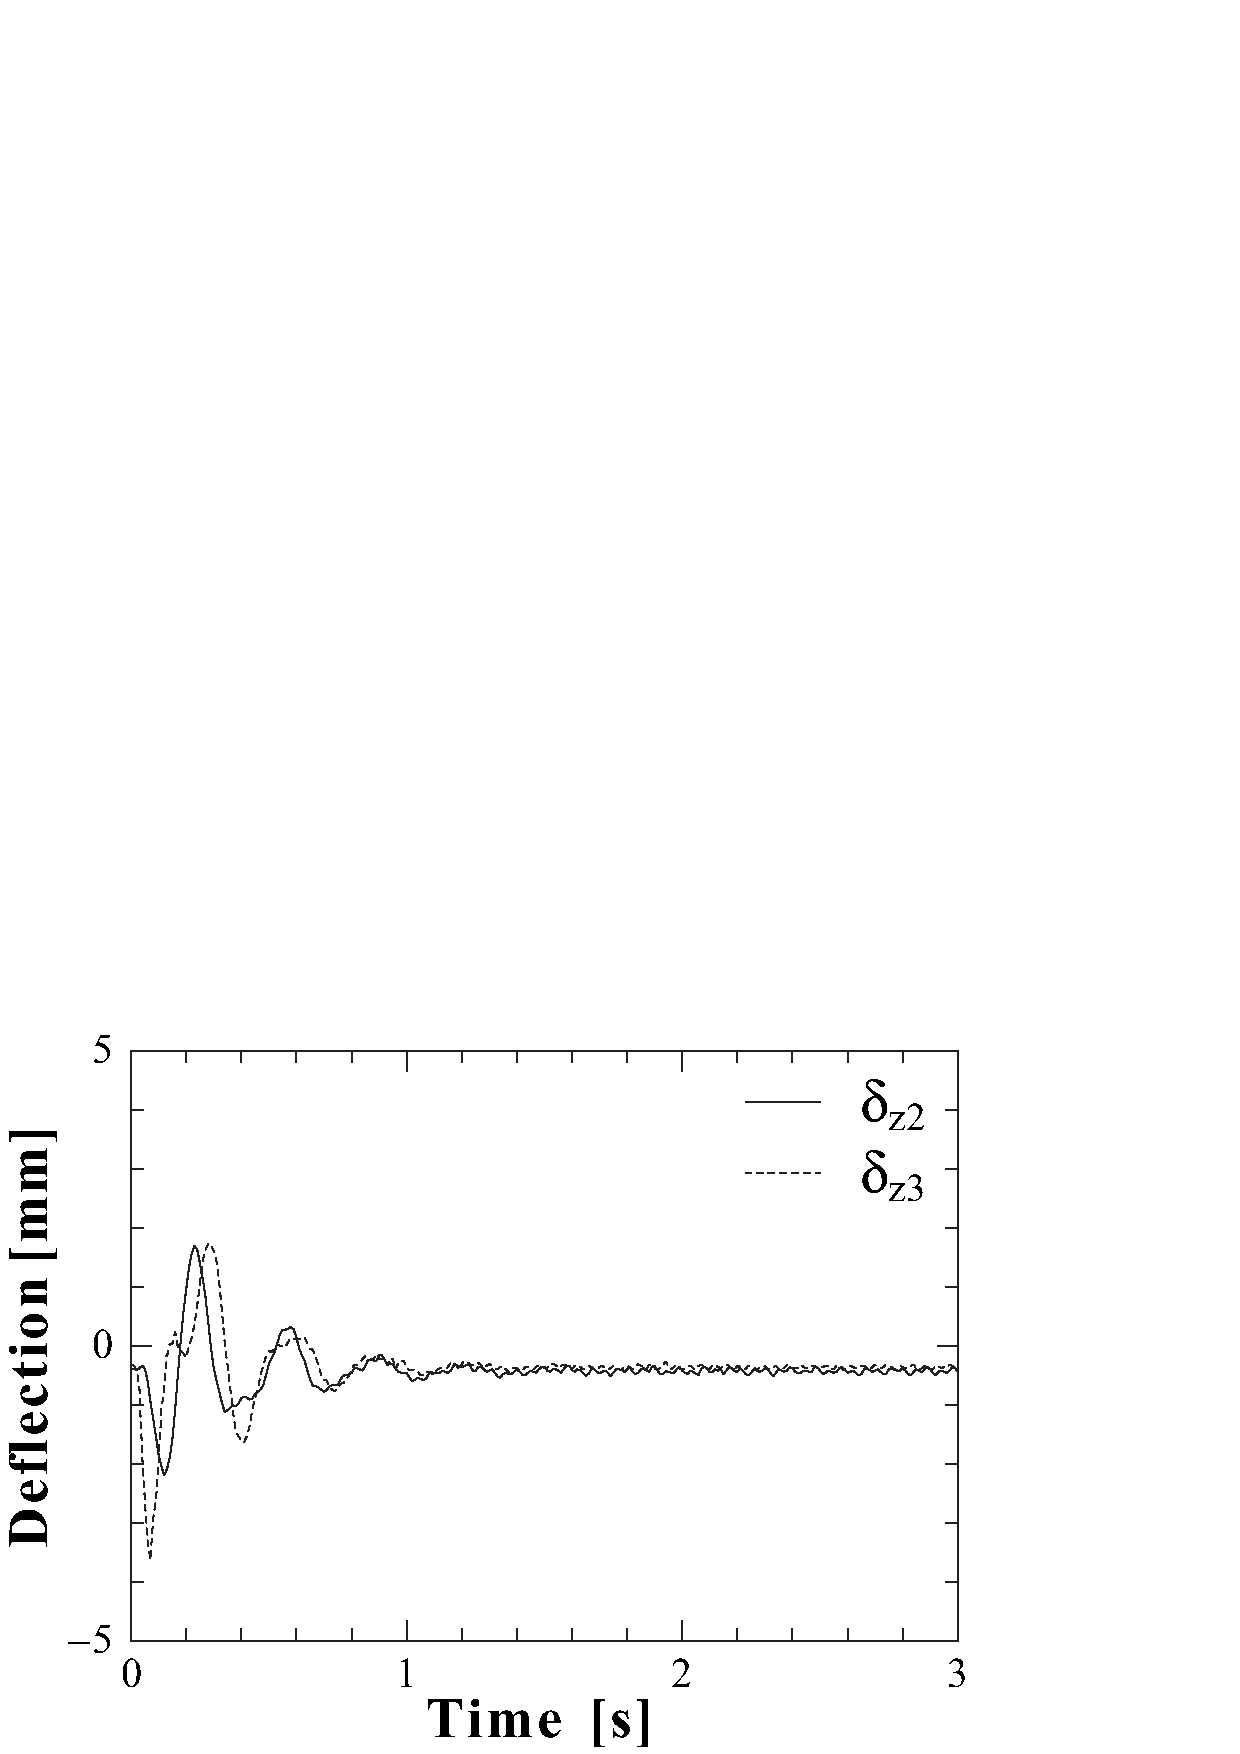
\includegraphics{fig1.png}}
% % \caption{Example of a figure caption.}
% % \label{fig}
% % \end{figure}

% Figure Labels: Use 8 point Times New Roman for Figure labels. Use words 
% rather than symbols or abbreviations when writing Figure axis labels to 
% avoid confusing the reader. As an example, write the quantity 
% ``Magnetization'', or ``Magnetization, M'', not just ``M''. If including 
% units in the label, present them within parentheses. Do not label axes only 
% with units. In the example, write ``Magnetization (A/m)'' or ``Magnetization 
% \{A[m(1)]\}'', not just ``A/m''. Do not label axes with a ratio of 
% quantities and units. For example, write ``Temperature (K)'', not 
% ``Temperature/K''.

% \section*{Acknowledgment}

% The author would like to thank Prof. Takadama, Assoc. Prof. Sato, 

% \section*{References}

% Please number citations consecutively within brackets \cite{b1}. The 
% sentence punctuation follows the bracket \cite{b2}. Refer simply to the reference 
% number, as in \cite{b3}---do not use ``Ref. \cite{b3}'' or ``reference \cite{b3}'' except at 
% the beginning of a sentence: ``Reference \cite{b3} was the first $\ldots$''

% Number footnotes separately in superscripts. Place the actual footnote at 
% the bottom of the column in which it was cited. Do not put footnotes in the 
% abstract or reference list. Use letters for table footnotes.

% Unless there are six authors or more give all authors' names; do not use 
% ``et al.''. Papers that have not been published, even if they have been 
% submitted for publication, should be cited as ``unpublished'' \cite{b4}. Papers 
% that have been accepted for publication should be cited as ``in press'' \cite{b5}. 
% Capitalize only the first word in a paper title, except for proper nouns and 
% element symbols.

% For papers published in translation journals, please give the English 
% citation first, followed by the original foreign-language citation \cite{b6}.

\begin{thebibliography}{00}
\bibitem{Niching}
S. W. Mahfoud, A comparison of parallel and sequential niching methods, in \textit{Proc. 6th Int. Conf. Genet. Algorithms}, pp.136-143, 1995.

% \bibitem{GA}
% M. Srinivas, L. M. Patniak, Genetic Algorithms: A Survey, \textit{Computer}, Vol.27, No.6, 17-26, 1994.

\bibitem{EAs01}
G. Singh and K. Deb, Comparison of Multi-modal Optimization Algorithms Based on Evolutionary algorithms., \textit{In Proceedings of the 8th Annual Conference on Genetic and Evolutionary Computation.}, 1305-1312, 2006.
% \bibitem{PSO01}
% R. Eberhart, J. Kennedy: A New Optimizer Using Particle Swarm Theory,
% \textit{Proc. Sixth International Symposium on Micro Machine and Human Science (Nagoya, Japan), IEEE Service center, Pis-cataway, NJ}, No.~1, pp.~39--43, 1995.

\bibitem{GAS}
D. E. Goldberg and J. Richardson, Genetic Algorithms with Sharing for Multimodal Function Optimization, in \textit{Proc. Genetic Algorithms Their Applicat. Conf.,}, pp.41-49, 1987.

\bibitem{EAs02}
R. K. Ursem, Multinational evolutionary algorithms, in \textit{Proc. Congr.Evol. Comput.(CEC)}, vol.3., pp.1633-1640, 1999.

\bibitem{DE}
R. Storn, K. Price, Differential Evolution − A simple and efficient adaptive scheme for global optimization over continuous spaces, Journal of global optimization, Vol.11, No.4, 341-359, 1997.

\bibitem{CDE}
R. Thomsen,"Multimodal Optimization using Crowding-based Differential Evolution," {\it In the IEEE Congress on Evolutionary Computation,}2004. CEC2004, vol.2, pp. 1382-1389, 19-23 June, 2004.

\bibitem{SDE}
X. Li, Efficient Differential Evolution using Speciation for Multimodal Function Optimization, \textit{In Proceedings of the Conference on genetic and evolutionary computation}, (GECCO'05), 873-880, 2005. 

% \bibitem{FA01}
% X. S. Yang: Firefly Algorithms for Multimodal Optimization,
% \textit{in:Stochastic Algorithms: Foundations and Applications, SAGA}, Vol.~5792, pp.~169--178, 2009.

\bibitem{BA01}
X. S. Yang: A Metaheuristic Bat-Inspired Algorithm,
 \textit{in: Nature Inspired Cooperative Strategies for Optimization(NICSO 2010), Springer, Berlin}, Vol.~284, pp.~65--74, 2010.

\bibitem{Niche} D.Beasley, D.R. Bull, and R.R. Martin, "A sequantial niche technique for multimodal function optimization," {\it Evolutionary Computation}, vol. 1, no.2, pp. 101-125,1993.

\bibitem{DNCMA}
O. M. Shir, T. Back: Dynamic niching in evolution strategies with covariance matrix adaption. \textit{In: Proceedings of the 2005 Congress on Evolutionary Computation(CEC2005)}, Piscataway, NJ, USA, IEEE Press (2005)
% \bibitem{f1}
% M. Molga, and C. Smutnicki, Test functions for optimization needs (2005). Retrieved June 2013, from \url{http://www.zsd.ict.pwr.wroc.pl/files/docs/functions.pdf.}

% \bibitem{f2}
% H. Pohlheim, GEATbx Examples: Examples of Objective Functions (2005). Retrieved June 2013, from \url{http://www.geatbx.com/download/GEATbx_ObjFunExpl_v37.pdf.}

\bibitem{NSBA}
 T. Iwase, R. Takano, F. Uwano, H. Sato and K. Takadama, "Novelty Search-based Bat Algorithm: Adjusting Distance among Solutions for Multimodal Optimization", {\it Proceedings of The 22nd Asia Pacific Symposium on Intelligent and Evolutionary Systems (IES 2018)}, pp.29--34, 2018. 

\bibitem{cec2013}
X. Li, A. Engelbrecht, and M. G. Epitropakis, "Benchmark Functions for CEC'2013 Special Session and Competition on Niching Methods for Multimodal Function Optimization", {\it Evol. Comput.} Mach. Learn. Group, RMIT University, Melbourne, VIC, Australia, Tech. Rep., 2013.
\end{thebibliography}
% \vspace{12pt}
% \color{red}
% IEEE conference templates contain guidance text for composing and formatting conference papers. Please ensure that all template text is removed from your conference paper prior to submission to the conference. Failure to remove the template text from your paper may result in your paper not being published.

\end{document}
